\documentclass{article}
    \usepackage[utf8]{inputenc}
    \usepackage[T1]{fontenc}
    \usepackage{tikz}
    \usepackage{xcolor}
    \usepackage{caption}
    \usepackage{amsmath}

    \definecolor{skyblue}{RGB}{135,206,235}
    \definecolor{brightmaroon}{RGB}{195, 33, 72}

    \usetikzlibrary{arrows.meta, shapes, positioning, matrix}

    \begin{document}

    \begin{figure}[htbp]
        \centering
        \resizebox{.45\linewidth}{!}{
            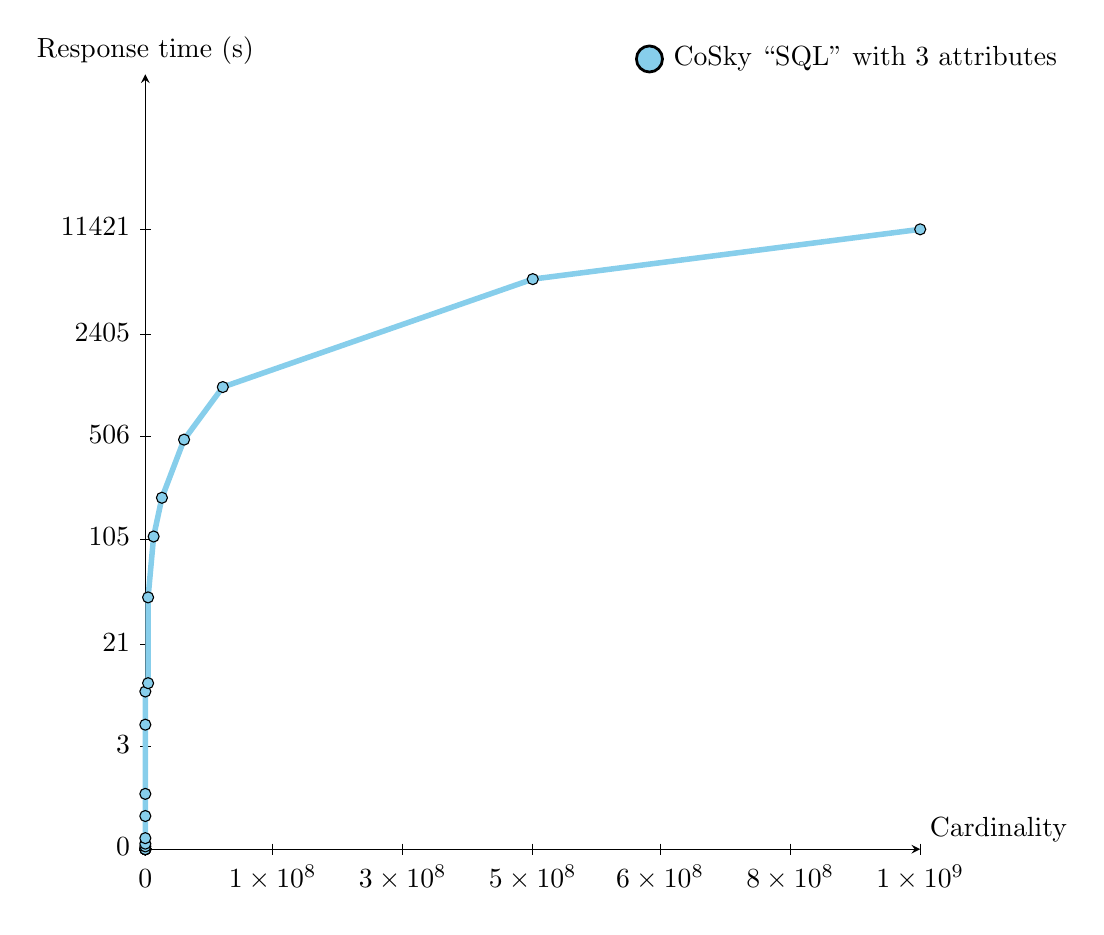
\begin{tikzpicture}[
                line join=bevel,
                bigcyannode/.style={shape=circle, fill=cyan, draw=black, line width=1pt},
                bigskybluenode/.style={shape=circle, fill=skyblue, draw=black, line width=1pt}
            ]
                % Axes
                \draw[-stealth] (0pt, 0pt) -- (280pt, 0pt) node[anchor=north west, yshift=15pt] {Cardinality};
                \draw[-stealth] (0pt, 0pt) -- (0pt, 280pt) node[anchor=south] {Response time (s)};

                % X-axis ticks
                \foreach \x/\xtext in {
                0pt/$0$,
                46pt/$1 \times 10^{8}$,
                93pt/$3 \times 10^{8}$,
                140pt/$5 \times 10^{8}$,
                186pt/$6 \times 10^{8}$,
                233pt/$8 \times 10^{8}$,
                280pt/$1 \times 10^{9}$} {
                \draw (\x, 2pt) -- (\x, -2pt) node[below] {\xtext\strut};
            }

            % Y-axis ticks
            \foreach \y/\ytext in {
                0pt/$0$,
                37pt/$3$,
                74pt/$21$,
                112pt/$105$,
                149pt/$506$,
                186pt/$2405$,
                224pt/$11421$} {
                \draw (2pt, \y) -- (-2pt, \y) node[left] {\ytext\strut};
            }

            % Curve and points
            \draw[skyblue, line width=2pt] (0pt, 0pt) -- (0pt, 0pt) -- (0pt, 0pt) -- (0pt, 0pt) -- (0pt, 0pt) -- (0pt, 0pt) -- (0pt, 0pt) -- (0pt, 0pt) -- (0pt, 0pt) -- (0pt, 1pt) -- (0pt, 2pt) -- (0pt, 4pt) -- (0pt, 12pt) -- (0pt, 20pt) -- (0pt, 45pt) -- (0pt, 57pt) -- (1pt, 60pt) -- (1pt, 91pt) -- (3pt, 113pt) -- (6pt, 127pt) -- (14pt, 148pt) -- (28pt, 167pt) -- (140pt, 206pt) -- (280pt, 224pt);
            \filldraw[color=black, fill=skyblue] (0pt, 0pt) circle (2pt);
            \filldraw[color=black, fill=skyblue] (0pt, 0pt) circle (2pt);
            \filldraw[color=black, fill=skyblue] (0pt, 0pt) circle (2pt);
            \filldraw[color=black, fill=skyblue] (0pt, 0pt) circle (2pt);
            \filldraw[color=black, fill=skyblue] (0pt, 0pt) circle (2pt);
            \filldraw[color=black, fill=skyblue] (0pt, 0pt) circle (2pt);
            \filldraw[color=black, fill=skyblue] (0pt, 0pt) circle (2pt);
            \filldraw[color=black, fill=skyblue] (0pt, 0pt) circle (2pt);
            \filldraw[color=black, fill=skyblue] (0pt, 0pt) circle (2pt);
            \filldraw[color=black, fill=skyblue] (0pt, 1pt) circle (2pt);
            \filldraw[color=black, fill=skyblue] (0pt, 2pt) circle (2pt);
            \filldraw[color=black, fill=skyblue] (0pt, 4pt) circle (2pt);
            \filldraw[color=black, fill=skyblue] (0pt, 12pt) circle (2pt);
            \filldraw[color=black, fill=skyblue] (0pt, 20pt) circle (2pt);
            \filldraw[color=black, fill=skyblue] (0pt, 45pt) circle (2pt);
            \filldraw[color=black, fill=skyblue] (0pt, 57pt) circle (2pt);
            \filldraw[color=black, fill=skyblue] (1pt, 60pt) circle (2pt);
            \filldraw[color=black, fill=skyblue] (1pt, 91pt) circle (2pt);
            \filldraw[color=black, fill=skyblue] (3pt, 113pt) circle (2pt);
            \filldraw[color=black, fill=skyblue] (6pt, 127pt) circle (2pt);
            \filldraw[color=black, fill=skyblue] (14pt, 148pt) circle (2pt);
            \filldraw[color=black, fill=skyblue] (28pt, 167pt) circle (2pt);
            \filldraw[color=black, fill=skyblue] (140pt, 206pt) circle (2pt);
            \filldraw[color=black, fill=skyblue] (280pt, 224pt) circle (2pt);

                % Legend
                \matrix [below left, draw=none] at (current bounding box.north east) {
                    \node [bigskybluenode, label=right:CoSky ``SQL'' with 3 attributes] {}; \\
                };
            \end{tikzpicture}
        }
        \caption{CoSky SQL: response time for 3 attributes}
        \label{fig:cosky_sql_response_time_3_attributes}
    \end{figure}

    \end{document}
    